\documentclass[sigconf]{acmart}

%\usepackage[T1]{fontenc}
\usepackage{lmodern}
\usepackage{abstract}
\usepackage{booktabs} % For formal tables
\usepackage{listings}
\usepackage{color}
\usepackage{multirow}
% For algorithms in ACM template
\usepackage[linesnumbered,ruled,vlined]{algorithm2e}

\definecolor{dkgreen}{rgb}{0,0.6,0}
\definecolor{gray}{rgb}{0.5,0.5,0.5}
\definecolor{mauve}{rgb}{0.58,0,0.82}

\lstset{frame=tb,
  language=C,
  aboveskip=3mm,
  belowskip=3mm,
  showstringspaces=false,
  columns=flexible,
  basicstyle={\small\ttfamily},
  numbers=none,
  numberstyle=\tiny\color{gray},
  keywordstyle=\color{blue},
  commentstyle=\color{dkgreen},
  stringstyle=\color{mauve},
  breaklines=true,
  breakatwhitespace=true,
  tabsize=3
}


% Copyright
%\setcopyright{none}
%\setcopyright{acmcopyright}
%\setcopyright{acmlicensed}
\setcopyright{rightsretained}
%\setcopyright{usgov}
%\setcopyright{usgovmixed}
%\setcopyright{cagov}
%\setcopyright{cagovmixed}


%% DOI
\acmDOI{}

%% ISBN
\acmISBN{}

%Conference info
\acmConference[CMSC 199]{CMSC 199}{May 2018}{Baguio City, Philippines} 
\acmYear{2018}
\copyrightyear{2018}

\acmPrice{0.00}

\newcommand*\LSTfont{\ttfamily\SetTracking{encoding=*}{-60}\lsstyle}

\begin{document}

\title{A Comparative Study on Brute Force, Boyer-Moore, and Berry Ravindran Pattern Matching Algorithms}
%\titlenote{Produces the permission block, and copyright information}
%\subtitle{Extended Abstract}
%\subtitlenote{The full version of the author's guide is available as \texttt{acmart.pdf} document}
\author{Deo Fetalvero}
\affiliation{%
  \institution{University of the Philippines Baguio}
  \streetaddress{Governor Pack Rd}
  \city{Baguio City} 
  \state{} 
  \postcode{2600}
}
\email{dmfetalvero@up.edu.ph}

\author{Paul Naraval}
\affiliation{%
  \institution{University of the Philippines Baguio}
  \streetaddress{Governor Pack Rd}
  \city{Baguio City} 
  \state{} 
  \postcode{2600}
}
\email{pdnaraval@up.edu.ph}

\author{Marielle Nolasco}
\affiliation{%
  \institution{University of the Philippines Baguio}
  \streetaddress{Governor Pack Rd}
  \city{Baguio City} 
  \state{} 
  \postcode{2600}
}
\email{mtnolasco@up.edu.ph}


\maketitle


% The default list of authors is too long for headers}
%\renewcommand{\shortauthors}{B. Trovato et al.}


\begin{abstract}
This paper discusses and compares three fundamental pattern matching algorithms: brute force, Boyer-Moore, and Berry Ravindran.
%\footnote{This is an abstract footnote}. 
\end{abstract}

%
% The code below should be generated by the tool at
% http://dl.acm.org/ccs.cfm
% Please copy and paste the code instead of the example below. 
%
%\begin{CCSXML}
%<ccs2012>
% <concept>
%  <concept_id>10010520.10010553.10010562</concept_id>
%  <concept_desc>Computer systems organization~Embedded systems</concept_desc>
%  <concept_significance>500</concept_significance>
% </concept>
% <concept>
%  <concept_id>10010520.10010575.10010755</concept_id>
%  <concept_desc>Computer systems organization~Redundancy</concept_desc>
%  <concept_significance>300</concept_significance>
% </concept>
% <concept>
%  <concept_id>10010520.10010553.10010554</concept_id>
%  <concept_desc>Computer systems organization~Robotics</concept_desc>
%  <concept_significance>100</concept_significance>
% </concept>
% <concept>
%  <concept_id>10003033.10003083.10003095</concept_id>
%  <concept_desc>Networks~Network reliability</concept_desc>
%  <concept_significance>100</concept_significance>
% </concept>
%</ccs2012>  
%\end{CCSXML}
%
%\ccsdesc[500]{Computer systems organization~Embedded systems}
%\ccsdesc[300]{Computer systems organization~Redundancy}
%\ccsdesc{Computer systems organization~Robotics}
%\ccsdesc[100]{Networks~Network reliability}

% We no longer use \terms command
%\terms{Theory}

%\keywords{ACM proceedings, \LaTeX, text tagging}


\section{Introduction}
 Pattern matching is an important concept in computer science due to its many technological applications such as DNA matching, voice recognition, face recognition, network security, and text processing.\cite{fsw}
\\
Pattern matching is finding one or all occurrences of a certain pattern $p$ of length $m$ in a text $t$ of length $n$. \cite{fsw} Pattern matching algorithms as is with all other algorithms base its performance by its time complexity. The time complexity of a pattern matching algorithm is based on its basic operation: comparison. A higher number of comparisons mean larger time complexity.\cite{fsw} Thus, most pattern matching algorithms are concerned with minimizing the number of comparisons to get a better time efficiency.
\\
This paper is concerned with discussing and illustrating three pattern matching algorithms: brute force, Boyer-Moore, and Berry Ravindran. 
\section{Definition of Terms}

\begin{itemize}
	\item Text: a body of characters $T$ to be matched upon.
	\item Pattern: a string of characters $P$ which is to be matched with the text.
  \item Window: the current position $k$ which $T[k+1]\ldots T[k+m]$ is aligned with $P[1]\ldots P[m]$, where $m$ is the length of pattern $P$.
  \item Mismatch: when the characters $T[k+1]\ldots T[k+m]$ does not match with all of $P[1]\ldots P[m]$.
\end{itemize}

\section{Brute Force}
The brute force or naive method compares each character in the pattern $p$ to each character in the text $t$. It compares $p$ to $t$ from left to right until it finds $p$ or a mismatch occurs or there is an insufficient number of characters left in $t$. \cite{berry}
\subsection{Algorithm}\cite{bruteforce}
The algorithm for the brute force method is given below:
\begin{lstlisting}
BruteForceStringMatch(T[0...n-1],P[0...m-1])
//Input: An array T[0...n-1] of n characters representing a text and an array P[0...m-1] of m characters representing a pattern
//Output: The index of the first character in the text that starts a matching substring or -1 if the search is unsuccessful
		for i = 0 to n-m do
			j = 0
			while j < m and P[j] = T[i+j] do
				j = j+1
			if j = m return i
		return -1 
\end{lstlisting} 
\subsection{Example}
As an example, let $T[0...n-1]=$ ''WE WANT TO EAT MORE ONIONS'', with whitespace being included, and $P[0...m-1]=$ ''ONION''.


\begin{lstlisting}[mathescape=true, basicstyle=\LSTfont]
text:  WE WANT TO EAT MORE ONIONS
pat:   ONION
       $\uparrow$
\end{lstlisting}

Since $T[0] = W \neq O = P[0]$, the pattern is immediately shifted to the right without further comparison.

\begin{lstlisting}[mathescape=true, basicstyle=\LSTfont]
text:  WE WANT TO EAT MORE ONIONS
pat:    ONION
        $\uparrow$
\end{lstlisting}

Similarly with $T[1+0] = T[1] = E \neq O = P[0]$, the pattern is shifted to the right. The same process goes on until a match is found in $i=20$.

\begin{lstlisting}[mathescape=true, basicstyle=\LSTfont]
text:  WE WANT TO EAT MORE ONIONS
pat:                       ONION
                           $\uparrow\uparrow\uparrow\uparrow\uparrow$
\end{lstlisting}

\subsection{Worst Case}\cite{bfworst}    
The worst case occurs when the number of comparisons is maximized. From the algorithm above, the maximum number of comparisons made between each character from $p$ to the characters in text $t$ is $m$. This is attained when each character from $p$ is compared to each corresponding character in $t$. Furthermore, the maximum number of comparisons between $p$ and $t$ is $n-m+1$. This is attained due to the nature of the algorithm wherein it compares $p$ to $t$ at least once and shifting just once if a mismatch occurs. Thus, the maximum number of comparison is $(m)(n-m+1)$ which implies that the time complexity of the worst case is $\Theta(nm)$.

\section{Heuristic Functions}
In Computer Science, A.I. and Mathematical optimizations, a heuristic function is a function that takes the best alternative out of one or more alternatives at a branching step in an algorithm. A heuristic function's objective is to speed up an algorithm by leading it to a `shortcut.' In some extreme cases these functions may not even improve the speed at which the algorithm converges to a solution and may add unnecessary load for the algorithm. A heuristic function may trade-off optimality, completeness, accuracy and precision depending on the implementation and objectives, in other cases heuristic functions may be generally benficial to the algorithm itself. \\

The following two exact string matching algorithms that will be discussed use heuristic functions to speed up the matching process.

\section{Boyer-Moore}		%	Boyer Moore
The Boyer-Moore String Matching algorithm performs its match from right to left instead the usual left to right of its time. This right to left matching enabled Boyer-Moore algorithm to skip more characters than the other algorithms\cite{boyerMoore}.

In Boyer-Moore string searching algorithm, the pattern $pat[1 ... patlen]$ of length $patlen$ is searched in string $string[1 ... stringlen]$ of length $stringlen$. For this part of the paper, let $char$ be defined as the $patlen^{th}$ character of $string$ when $pat$ is placed on top of the leftmost part of $string$ - $char$ is the character of $string$ aligned with the last character of $pat$. Boyer and Moore uses a function to quickly traverse $string$. It is the Bad Character Shift, which was initially referred to as $delta_1$.\cite{boyerMoore}

\subsection{Algorithm}
\cite{boyerMoore}The Boyer-Moore searches using the following algorithm:
\begin{lstlisting}[mathescape=true]
		$stringlen \gets$ length of $string$.
		$i \gets patlen.$
$top$:	if $i > stringlen$ then return false
		$j \gets patlen$.
$loop$:	if $j=0$ then return $j+1$.
		if $string(i)=pat(j)$
			then
			$j \gets j-1$.
			$i \gets i-1$.
			goto $loop$.
			close;
		$i \gets i + badChar(\ string(i)\ )$
		goto $top$
\end{lstlisting}

The function $badChar$ is defined by Boyer and Moore as\\

\begin{equation*}
  badChar =
  \begin{cases}
    patlen & \text{does not occur in $patlen$} \\
    2*patlen-j & \text{otherwise; where $pat(j)$ is the} \\
     & \text{rightmost occurrence of $char$ in $pat$}
  \end{cases}
\end{equation*}

\subsection{Example}
To make this algorithm clearer, the same example as before will be used.
\begin{lstlisting}[mathescape=true, basicstyle=\LSTfont]
string:  WE WANT TO EAT MORE ONIONS
pat:     ONION
             $\uparrow$
\end{lstlisting}

As $string[5]=$A is not in the pattern, $pat$ is shifted by $patlen=5$ to the right.

\begin{lstlisting}[mathescape=true, basicstyle=\LSTfont]
string:  WE WANT TO EAT MORE ONIONS
pat:          ONION
                  $\uparrow$
\end{lstlisting}

This time $string[10]=$O can be found in $pat$ with the rightmost occurrence at $j=4$. Hence the pattern is shifted to the right by $5-4=1$.

\begin{lstlisting}[mathescape=true, basicstyle=\LSTfont]
string:  WE WANT TO EAT MORE ONIONS
pat:           ONION
                   $\uparrow$
\end{lstlisting}

This setting is done until $i=25$

\begin{lstlisting}[mathescape=true, basicstyle=\LSTfont]
text:  WE WANT TO EAT MORE ONIONS
pat:                       ONION
                           $\uparrow\uparrow\uparrow\uparrow\uparrow$
\end{lstlisting}

\subsection{Worst Case}
The worst case of Boyer-Moore algorithm occurs when for every alignment $pat[1...patlen]$ and $string[i-patlen+1...i]$, every element is compared with only the first elements not being equal. Hence per alignment, $patlen$ comparisons will be done. Also, the pattern is only shifted to the right by one. Since $string$ has the length $stringlen$ and $pat$ is $patlen$ long, there will be $(stringlen-patlen+1)$ alignments. Therefore, the maximum number of comparisons is $(patlen)\times(stringlen-patlen+1)$, consequently it has a complexity of $\Theta\left(patlen \times stringlen\right)$.\cite{berry}


\section{Berry-Ravindran}			%	Berry-Ravindran
Based on a plethora of algorithms that was brought about by Boyer-Moore Exact String Matching Algorithm, Berry and Ravindran designed an algorithm which does shifting considering the two consecutive characters to the right of the window.
\subsection{Algorithm}
\begin{enumerate}
\item Let $P$ be the pattern string to find. Let $T$ be the text to be matched upon. Let $n$ be the length of text $T$ where $T[1]$ is the first character and $T[n]$ is the last character of text $T$. Let $m$ be the length of the pattern such that $P[m]$ is the last character and $P[1]$ is the first character of pattern $P$.

\item Create and initialize the Shift Table. The two dimensional array, $ST$ (Shift Table), of size at most $(m+1)\times(m+1)$ will store the shift values for all pairs of characters. The $ST$ will be initialised with values of $m+2$.

\item Create and fill the $CON$ Table. As the index of the $ST$ is of type integer, we need to convert the pairs of characters into pairs of integers. This is done by defining an array of ASCII character set size called $CON$ with each entry initialised to $0$.

\item For each character $c$ in the pattern the right most position (numbering from the right, starting with 1) is entered in the corresponding location in $CON$ ($CON[c]=$ right most position of c).

\item For every index $i$ starting at $1$, reading from left to right and finish at $m+1$, do steps 6-9.

	\item For each of characters $P[i]$ and $P[i-1]$ find the values of indices $a$ and $b$ from $CON[P[i-1]]$ and $CON[P[i]]$ respectively, in the $CON$ table. If any of $P[i]$ or $P[i-1]$ does not exist, for every index $q$ available to $ST$ table, set $b=q$ or $a=q$, respectively and do step 7 otherwise, if both exist, proceed.

	\item In the shift table $ST$ at $(a, b)$, set the value with the formula: $$ ST(a,b) = m+2-i $$

\item Create the index $k$. Set a new variable $k=0$.

\item For every character $P[i]$ (index $i$) starting at $P[m]$ (index $m$) and finishing at $P[1]$ (index $1$), do step 10 
	
	\item Compare the characters $P[i]$ with $T[k + i]$. If they're not the same (mismatch), skip to step 11. If they're the same, continue searching and once each pairs of characters are all the same, declare a match at $T[k+1]$ to $T[k+m]$ and stop the program.

\item Find the shift value $s$. The value of a shift for the pair $T [k +m+ 1]$ and $T [k +m+ 2]$ is $s = ST (CON[T[k + m+ 1]], CON[ T [k +m+ 2]])$. 
	
\item Add the new shift value to $k$. Set $k=k+s$.

\item Check the alignment window. Check if the new $k+m > n$. If true, declare that no match was found and stop the program, otherwise repeat steps 10-14. 

\end{enumerate}
\subsection{Example}
For an example, the pattern `onion' is tested with the text `we want to test with onion'. The example is referenced to Thomas Berry's Dissertation \cite{berry}. 
Let $P$ be the pattern `onion' and $T$ be the text `we want to test with onion'. Now let $m$ be the length of the pattern which is $5$ and $n$ be the length of the text which is $26$. Further, the $CON$ table is generated as follows:

\begin{center}
\begin{tabular}{ c c c c c c c c }
 Character & \ldots & a & b & \ldots & h & i & j \\ 
 ASCII Value & \ldots & 97 & 98 & \ldots & 104 & 105 & 106 \\  
 CON & \ldots & 0 & 0 & \ldots & 0 & 3 & 0    
\end{tabular}
\end{center}

\begin{center}
\begin{tabular}{ c c c c c c c c }
 Character & \ldots & n & o & p & \ldots \\ 
 ASCII Value & \ldots & 110 & 111 & 112 & \ldots \\  
 CON & \ldots & 1 & 2 & 0 & \ldots   
\end{tabular}
\end{center}

The $ST$ table is all initialized with values of $m+2$ which is $7$. The Shift Values will be entered in the following order:
\begin{enumerate}
\item For $CON[$ (any) $]$ and $CON[$ o$]$, $ST($ (any) $,2) = 6$
\item For $CON[$n$]$ and $CON[$ i$]$, $ST(1,3) = 5$
\item For $CON[$i$]$ and $CON[$ o$]$, $ST(3,2) = 4$
\item For $CON[$o$]$ and $CON[$ n$]$, $ST(2,1) = 3$
\item For $CON[$o$]$ and $CON[$ n$]$, $ST(2,1) = 2$
\item For $CON[$n$]$ and $CON[$ (any) $]$, $ST(1, $ (any) $) = 1$
\end{enumerate}
The $ST$ table would look like the following after the values are entered. The table is accessed by row and then by column such that the value of $ST(i,j)$ of any $i$ or $j$ is at row $i$ and column $j$. \\

\begin{tabular}{ | c | c c c c | }
\toprule
    & 0 & 1 & 2 & 3  \\
\midrule
  0 & 7 & 7 & 6 & 7  \\
  1 & 1 & 1 & 1 & 1  \\
  2 & 7 & 2 & 6 & 7  \\
  3 & 7 & 7 & 3 & 7  \\
\bottomrule
\end{tabular}\\
 \\
The preprocessing section of the algorithm is now over. String matching can now be initiated. The $ST$ and $CON$ tables will now be used as a heuristic to speed up the string matching process.\\
In the following tables, the remaining steps are executed until a `match' or `no matches' declaration can be inferred. The first row shows the text and the third row shows the position of the pattern. The second row shows whether the aligned pattern and text characters match ($=$) or mismatch ($\neq$) as the comparisons are made.
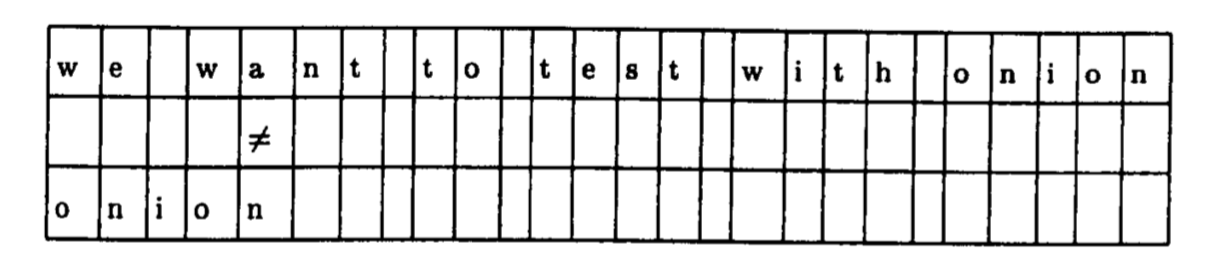
\includegraphics[width=0.5\textwidth]{img/br-1.png}
\captionof*{table}{Mismatch shift on $ST(CON[$n$], CON[$t$]) = ST(1,0) =1$}
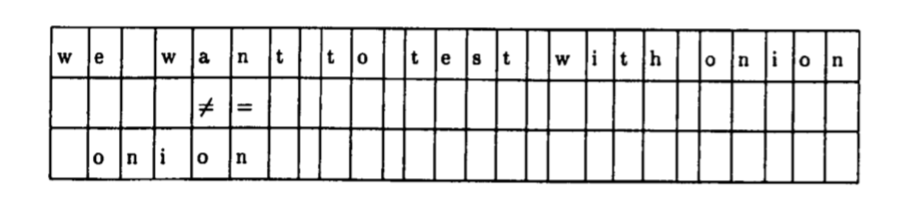
\includegraphics[width=0.5\textwidth]{img/br-2.png}
\captionof*{table}{Mismatch shift on $ST(Con [$t$],CON[$ $]) = ST(0,0) =7$}
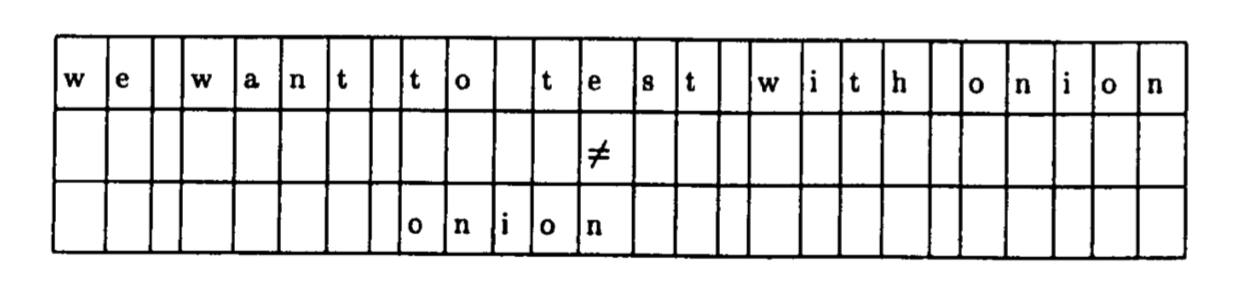
\includegraphics[width=0.5\textwidth]{img/br-3.png}
\captionof*{table}{Mismatch shift on $ST(Con [$s$],CON[$t$]) = ST(0,0) =7$}
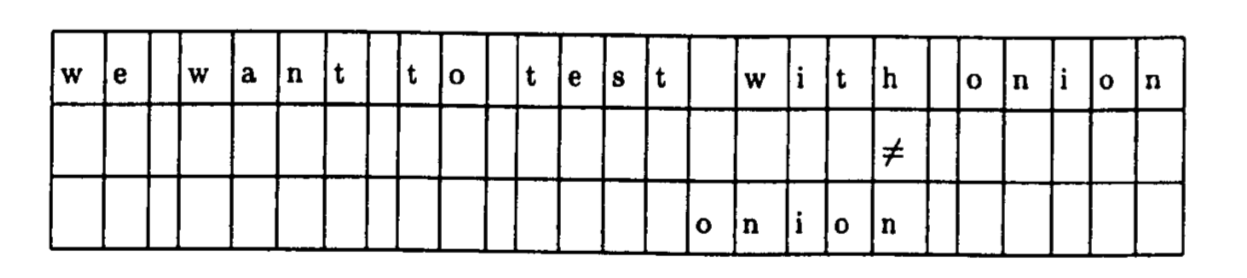
\includegraphics[width=0.5\textwidth]{img/br-4.png}
\captionof*{table}{Mismatch shift on $ST(Con [$ $],CON[$o$]) = ST(0,2) =6$}
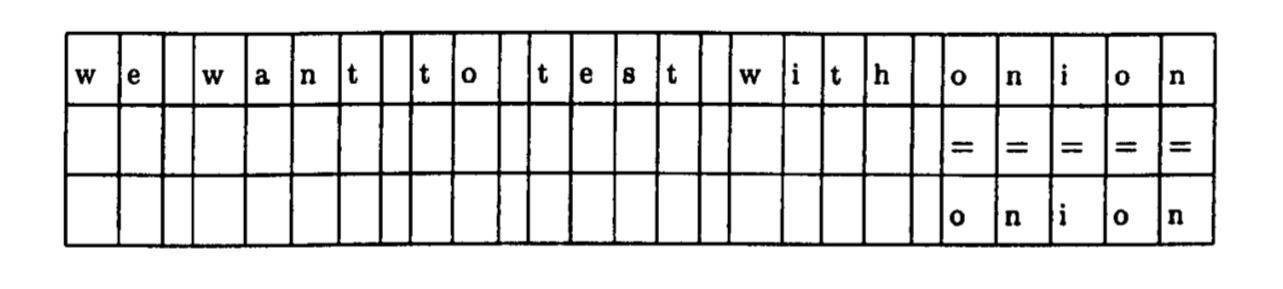
\includegraphics[width=0.5\textwidth]{img/br-5.png}
\captionof*{table}{So the pattern `onion' has been matched and the test is exhausted}

Further, the word `onion', in a text length of $26$, was found using only $10$ comparisons.


\bibliographystyle{ACM-Reference-Format}
\bibliography{bibliography}

\end{document}
